\pagebreak
\section{Moltiplicazione polinomiale}
\subsection{Esempio}
Dati due polinomi di $x$ di grado $N-1$,
\begin{equation*}
P  = \displaystyle\prod_{i=0}^{N-1} {a}_{i} {x}^{i},\,
        P' = \displaystyle\prod_{i=0}^{N-1} {b}_{i} {x}^{i},
        (a_i,b_i) \in (\mathbb{Z}_q, \mathbb{Z}_q)
\end{equation*}\\
prima di descrivere il prodotto modulo $q$, può essere utile considerare un
esempio concreto del loro prodotto con $(N, q) = (3, 10)$, introducendo come
notazione
`$+_q$' la somma in $\mathbb{Z}_q$,
`$\times_q$' il prodotto in $\mathbb{Z}_q$,
`$=_q$' l'equivalenza modulo $q$:
\\
\begin{table} [h]
    \begin{tabular} {rlllll|ll|l}
        $[x]$ &   &   & 1 & 2 & 3 &  &  & $\times_{10}$             \\ 
        $[x]$ &   &   & 4 & 5 & 6 &  &  & $=_{10}$                  \\ 
        \hline
        $[x]$ &   &   & 1 & 2 & 3 & $\times_{10}$ & 4 & $+_{10}$    \\
        $[x]$ &   & 1 & 2 & 3 & 0 & $\times_{10}$ & 5 & $+_{10}$    \\
        $[x]$ & 1 & 2 & 3 & 0 & 0 & $\times_{10}$ & 6 & $=_{10}$    \\
        \hline
        $[x]$ &   &   & 4 & 8 & 2 &  &  & $+_{10}$                  \\
        $[x]$ &   & 5 & 0 & 5 & 0 &  &  & $+_{10}$                  \\
        $[x]$ & 6 & 2 & 8 & 0 & 0 &  &  & $=_{10}$                  \\
        \hline
        $[x]$ & 6 & 7 & 2 & 3 & 2 &  &  &
    \end{tabular}
\end{table}\\
È possibile notare che il prodotto polinomiale abbia la classica struttura
della moltiplicazione in colonna senza propagazione del carry, dato che
$10=_{10}0$.\\
\subsection{Definizione}
Introducendo quindi la formula di prodotto polinomiale\\
\begin{equation*}
    P {\times}_q P'                                                     =
        {\displaystyle\sum_{i=0}^{N-1}}_q P(j - i) {\times}_q P'(i)     =
        {\displaystyle\sum_{i=0}^{j}}_q P(i) {\times}_q  P'(N - 1 - j)
\end{equation*}
\\
appare noto che il prodotto polinomiale da luogo alla convoluzione delle
sequenze dei coefficienti dei due polinomi, ed è dunque possibile fare uso
della trasformata di Fourier in $\mathbb{Z}_q$, per introdurre un notevole
incremento delle performace, sfruttando la seguente proprietà:
\begin{equation}
    \label{Mulfft}
    S \otimes S' =
    \mathrm{IFFT}_{2N} ( { \mathrm{FFT}_{2N} S \times \mathrm{FFT}_{2N} S' } )
\end{equation}
\pagebreak
\\
\section{Complessità operativa}
\subsection{Implementazione diretta}
Una stima accurata di una moltiplicazione polinomiale è molto difficile senza
una sua implementazione pratica.\\
\\
Data l'estrema ridondanza negli operandi nella funzione di convoluzione una
parte non trascurabile della massimizzazione delle performance in prezenza di
vettorizzazione consiste nella minimizzazione della comunicazione tra L1 cache
ai registri, rendendo due procedure che eseguono le medesime operazioni
algebriche estremamente diverse in termini di performance, basti pensare che
$c \gets a + b$ in una moderna architettura Intel, composta da due load
(4 cycles), una addizione (1 cycle) e 1 store (4 cycles), l'operazione
aritmetica di addizione costituisce del solo $11\%$ del carico della CPU.\\
\\
Tuttavia, dato il costo dominante del prodotto modulo q rispetto ad ogni altro
tipo di operazione, è possibile usare il numero di prodotti come proxy per le
performance dei due algoritmi, rimandando ad un'analisi più accurata della
complessità del prodotto al seguito della trattazione.\\
\\
La complessità stimata di un'implementazione diretta del prodotto di due
polinomi di grado $N-1$ è dunque di $O(N^2)$.\\
\pagebreak
\subsection{Implementazione con NTT}
Poiché la trasformata di Fourier a $2N$ punti
$\mathcal{F}_{2N} = \displaystyle\sum_{i=0}^{2N-1}a_i W_{2N}^{n i}$
equivale a valutare il polinomio nelle potenze delle radici dell'unità in
$\mathbb{Z}_q$ del tipo $W^i_{2N}$, mentre il quoziente $\langle x^N+1\rangle$
rimuove le soluzioni nelle radici con molteplicità \\
$W^n_N = W^{2n}_{2N}$, è sufficiente valutare il polinomio in
$W^{2i(n+1)}_{2N}$. Essendo
\begin{equation*}
    \displaystyle\sum_{i=0}^{N-1}a_i W_{2N}^{2i(n + 1)} =
    \displaystyle\sum_{i=0}^{N-1} (a_i W_N^{\frac{i}{2}}) W_{N}^{n i}
\end{equation*}
è possibile ridurre le $\mathrm{FFT}_{2N}$ a $\mathrm{FFT}_N$ del nuovo
polinomio con coefficienti $(a_i W_N^{\frac{i}{2}})$ al costo di $N$ prodotti
modulo $q$ sul totale delle operazioni. La $\mathrm{IFFT}_N$ soffre dello
stesso costo aggiuntivo, ma tale prodotto viene combinato con la
moltiplicazione per il fattore $N^{-1}$.\\
\\
È possibile perciò andare a stimare il costo della moltiplicazione come
\begin{equation*}
O(N) + 2(O(N) + O(\mathrm{FFT}) + O(\mathrm{IFFT})
\end{equation*}
direttamente dalla formula (\ref{Mulfft}), dove l'aggiuntivo $O(N)$ è dovuto ai
prodotti dei coefficienti membro a membro nello spazio trasformato.\\
\\
Il costo della $\mathrm{FFT}_N$, stimato attraverso il numero di moltiplicazioni modulo
q è di $O(\frac{N}{2}(log_2(N) - 1)$, questo perché la sua pipeline è composta
da $log_2(N)$ stadi, di cui solo gli ultimi $log_2(N) - 1$ generano prodotti
modulo $q$.\\
Ogni stadio è composto da $\frac{N}{2}$ strutture a farfalla, ognuna delle
quali contribuisce un prodotto.\\
\\
\tikzset {
    mem/.style={rectangle, fill=white, inner sep=1pt, font=\tiny},
    circ/.style={circle, draw=black, fill=white, inner sep=1pt, font=\tiny},
}
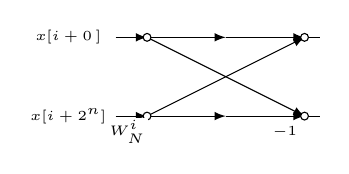
\begin{tikzpicture}
    \node at (-0.5, 0) [mem] {$x[i+2^n]$};
    \node at (-0.5, 1) [mem] {$x[i+0\,]$};
    \draw [->, >=latex] (.1, 0) -- (.5, 0);
    \draw [->, >=latex] (.5, 0) -- (1.5, 0);
    \draw [->, >=latex] (1.5, 0) -- (2.5, 0);
    \draw [->, >=latex] (.1, 1) -- (.5, 1);
    \draw [->, >=latex] (.5, 1) -- (1.5, 1);
    \draw [->, >=latex] (1.5, 1) -- (2.5, 1);
    \draw [->, >=latex] ((.5, 0) -- (2.5, 1);
    \draw [->, >=latex] ((.5, 1) -- (2.5, 0);
    \draw [] ((2.5, 1) -- (2.7, 1);
    \draw [] ((2.5, 0) -- (2.7, 0);
    \node at (.5, 0) [circ] {};
    \node at (.5, 1) [circ] {};
    \node at (2.5, 0) [circ] {};
    \node at (2.5, 1) [circ] {};
    \node at (0.25, -0.2) [mem] {$W^i_N$};
    \node at (2.25, -0.2) [mem] {$-1$};
\end{tikzpicture}\\
\\
Indicando con $W^i_N$ le radici dell'unità in $\mathbb{Z}_q$ è possibile notare
che per ogni stage esistono dei prodotti per $W^0_N$. Nonostante il risultato
di tali moltipilicazioni sia noto, queste operazioni non possono essere evitate
in un modello vettorizzato del codice, e vengono quindi incluse nel conteggio
della complessità.\\
\pagebreak
\\
La complessità della $\mathrm{IFFT}$ è di $O(\mathrm{FFT}) + O(N)$, dovuto ad
un ulteriore stage moltiplicativo in uscita per $N^{-1} W_N^{-\frac{i}{2}}$ in
$\mathbb{Z}_q$.\\
\\
La complessità finale dell'algoritmo di moltiplicazione polinomiale risulta
quindi essere $O(Nlog_2(N) + 3N)$. Per dei polinomi di $N=1024$ questo
ammonta a 13'312 prodotti, mentre per un implementazione diretta $O(N^2)$
ammonterebbe a 1'048'576 prodotti.\\
\\
Un'ultima considerazione sulle performance riguardano il tipo di decimazione
usato dalla $\mathrm{FFT}$: sebbene non compaia nel calcolo della comlessità il costo
operativo degli stage di bitreverse shuffle ammonta a più del $10\%$
dell'intera pipeline.\\
\\
Nel caso i coefficenti nel dominio trasformato siano necessari in ordine è
consigliato un algoritmo di decimazione nel tempo, essendo preferibili
unaligned cache reads a unaligned cache writes. Tuttavia è possibile utilizzare
una trasformata dei coefficienti dei due polinomi verso il dominio trasformato
con decimazione in frequenza , eseguire il prodotto mantenendo l'ordine
bireverse shuffled, ed antitrasformare con un tipo di decimazione nel tempo, in
modo da evitare le due operazioni intermedie di reverse shuffle.
\pagebreak
